\documentclass{article}

% Margins and spacing
\usepackage[a4paper, margin=.7in]{geometry}
% Math packages
\usepackage{amsmath}
\usepackage{amssymb}
% Figures and graphics
\usepackage{graphicx}
\usepackage{caption}
% Placement of figures, tables, algorithms, etc.
\usepackage{float}
% Hyperlinks
\usepackage{hyperref}
% Reference section names
\usepackage{nameref}
% Algorithms
\usepackage{algorithm}
\usepackage{algpseudocode}

%% Tips
% Fix spacing between lines
% \vspace{-\baselineskip}

% No section numbering
\setcounter{secnumdepth}{0}
% No page numbering
\pagenumbering{gobble}
% No paragraph indentation
\setlength{\parindent}{0pt}
% Removes caption prefixes (e.g., "Figure 1:") from figures
\captionsetup[figure]{labelformat=empty}

% Define custom commands
%% Underlined hyperlinks
\newcommand{\uhref}[2]{\href{#1}{\underline{#2}}}
%% Bold-italic math symbols
\newcommand{\mathbi}[1]{\boldsymbol{#1}}
%% Operators
\DeclareMathOperator*{\argmin}{arg\,min}
\DeclareMathOperator*{\argmax}{arg\,max}
\DeclareMathOperator{\sgn}{sgn}
%% Manually indented states in algorithmic environment
\newcommand{\IndentState}{\State \hspace{1em}}
\newcommand{\DIndentState}{\State \hspace{2em}}

\title{EE588: Homework 1 Solutions}
\author{
  Naman Chhibbar \\
  USC ID: 7709-8548-02
}
\date{}

% Document body
\begin{document}
\maketitle

\section{Textbook Exercises}
\begin{itemize}
  \item[2.2] Show that a set is convex if and only if its intersection with any line is convex. Show that a set is affine if and only if its intersection with any line is affine. \\

  \textbf{Solution:} Let $A$ be an affine set and $L$ be any line. If $A \cap L$ is empty or singleton, it will be affine by definition. Supose $A \cap L$ has at least two points, then the affine combination of the two points will also be in $A$ (since $A$ is affine), which is $L$. Therefore, $L \subseteq A$, making $A \cap L = L$ affine (lines are affine). \\
  Now suppose $A$ is any set such that $A \cap L$ is affine for any line $L$. Let $x_1, x_2 \in A$ and consider the line $L$ passing through them. Since $A \cap L$ is affine, $A \cap L = L$. Therefore $A$ contains affine combinations of any two points in $A$, making it affine. \\
  Now let $C$ be a convex set and $L$ be any line. If $C \cap L$ is empty or singleton, it will be convex by definition. Suppose $C \cap L$ has at least two points $x_1$ and $x_2$. Let $L_0$ be the convex combination of $x_1$ and $x_2$. Since both $C$ and $L$ are convex (all affine sets are convex), $L_0 \subseteq C$ and $L_0 \subseteq L$. Therefore, $L_0 \subseteq C \cap L$, making $C \cap L$ convex. \\
  Now suppose $C$ is any set such that $C \cap L$ is convex for any line $L$. Let $x_1, x_2 \in C$ and consider the line $L$ passing through them. Since $C \cap L$ is convex, $C \cap L$ contains the convex combination of $x_1$ and $x_2$. Hence, $C$ contains the convex combination of any two points in $C$, making it convex.

  \item[2.5] What is the distance between two parallel hyperplanes $\{x \in \mathbb{R}^n : a^T x = b_1\}$ and $\{x \in \mathbb{R}^n : a^T x = b_2\}$? \\
  
  \textbf{Solution:} Denote $H_1 = \{x \in \mathbb{R}^n : a^T x = b_1\}$ and $H_2 = \{x \in \mathbb{R}^n : a^T x = b_2\}$. Let $x_0 \in H_1$ and consider the point $x_0 + \lambda a$, where $\lambda \in \mathbb{R}$. If we find a $\lambda$ such that $x_0 + \lambda a \in H_2$, then the distance between the two hyperplanes will be $\|x_0 - (x_0 + \lambda a)\| = |\lambda| \cdot \|a\|$. We have:
  \[ a^T (x_0 + \lambda a) = b_2 \]
  \[ \Rightarrow a^T x_0 + \lambda a^T a = b_2 \]
  \[ \Rightarrow b_1 + \lambda \|a\|^2 = b_2 \]
  \[ \Rightarrow \lambda = \frac{b_2 - b_1}{\|a\|^2} \]
  Hence, the distance between the two hyperplanes is:
  \[ |\lambda| \cdot \|a\| = \frac{|b_2 - b_1|}{\|a\|} \]

  \item[2.7] \textit{Voronoi description of halfspace.} Let $a$ and $b$ be distinct points in $\mathbb{R}^n$. Show that the set of all points that are closer (in Euclidean norm) to $a$ than to $b$, i.e., $\{x \in \mathbb{R}^n : \|x - a\|_2 \leq \|x - b\|_2\}$, is a halfspace. Describe it explicitly as an inequality of the form $c^T x \leq d$. Draw a picture. \\
  
  \textbf{Solution:}
  \begin{align*}
    \|x - a\|_2 &\leq \|x - b\|_2 \\
    \Rightarrow \|x - a\|_2^2 &\leq \|x - b\|_2^2 \\
    \Rightarrow (x - a)^T (x - a) &\leq (x - b)^T (x - b) \\
    \Rightarrow x^T x - 2 a^T x + a^T a &\leq x^T x - 2 b^T x + b^T b \\
    \Rightarrow 2 (b - a)^T x &\leq b^T b - a^T a \\
    \Rightarrow c^T x &\leq d
  \end{align*}
  Where $c = 2 (b - a)$ and $d = b^T b - a^T a$. Hence, the given set defines a halfspace.

  \item[2.10] \textit{Solution set of a quadratic inequality.} Let $C \subseteq \mathbb{R}^n$ be the solution set of a quadratic inequality,
  \[ C = \{x \in \mathbb{R}^n : x^T A x + b^T x + c \leq 0\}, \]
  with $A \in \mathbb{S}^n$, $b \in \mathbb{R}^n$, and $c \in \mathbb{R}$.
  \begin{itemize}
    \item[(a)] Show that $C$ is convex if $A \succeq 0$.
    \item[(b)] Show that the intersection of $C$ and the hyperplane defined by $g^T x + h = 0$ (where $g \neq 0$) is convex if $A + \lambda g g^T \succeq 0$ for some $\lambda \in \mathbb{R}$.
  \end{itemize}
  Are the converses of these statements true? \\

  \textbf{Solution:}
  \begin{itemize}
    \item[(a)] Let $f(x) = x^T A x + b^T x + c$. Now:
    \begin{align*}
      \nabla f(x) &= 2 A x + b \\
      \Rightarrow \nabla^2 f(x) &= 2 A
    \end{align*}
    Since $A \succeq 0$, $\nabla^2 f(x) \succeq 0$ (scaling by a positive scalar retains the property). Hence, $f$ is convex. Let $x_1, x_2 \in C$ and $\theta \in [0, 1]$. By definition of $f$, we get $f(x_1) \leq 0$ and $f(x_2) \leq 0$. Since $f$ is convex, we have:
    \[ f(\theta x_1 + (1 - \theta) x_2) \leq \theta f(x_1) + (1 - \theta) f(x_2) \leq 0 \]
    Since $\theta$ and $(1 - \theta)$ are non-negative. Hence, $\theta x_1 + (1 - \theta) x_2 \in C$, making $C$ convex. \\
    And no, the converse is not true. Consider the case with $A = -I$, $b = 0$, and $c = -1$. Now, $f$ becomes:
    \[ f(x) = -x^T x - 1 = -\|x\|^2 - 1 \le 0 \]
    \[ \Rightarrow \|x\|^2 \ge -1 \]
    This is always true, so $C = \mathbb{R}^n$, which is convex. However, $A$ is not positive semidefinite.
    \item[(b)] Once again, let $f(x) = x^T A x + b^T x + c$. Denote the given hyperplane by $H$ and the intersection by $\tilde{C} = C \cap H$. Define $\tilde{f}(x) = f(x) + \lambda(g^T x + h)^2$. Note that $\tilde{f}(x) = f(x) \le 0$ for all $x \in \tilde{C}$ since $g^T x + h = 0$ for all $x \in \tilde{C} \subseteq H$. Now:
    \begin{align*}
      \tilde{f}(x) &= f(x) + \lambda (g^T x + h)^2 \\
      &= f(x) + \lambda (g^T x + h)(x^T g + h) \\
      &= f(x) + \lambda (x^T g g^T x + 2 h g^T x + h^2) \\
      &= x^T (A + \lambda g g^T) x + (b + 2 \lambda h g)^T x + (c + \lambda h^2) \\
      \Rightarrow \nabla^2 \tilde{f}(x) &= 2 (A + \lambda g g^T)
    \end{align*}
    Using the same argument as in part (a), the solution set of $\tilde{f}(x) \leq 0$ is convex. Note that the intersection of solution set of $\tilde{f}(x) \leq 0$ and $H$ is $\tilde{C}$, and since intersection of convex sets is also convex, we conclude that $\tilde{C}$ is convex. \\
    And again, the converse is not true. Consider a similar case as in part (a) with $A = -I$, $b = 0$, and $c = -1$ with $n = 2$. We know from part (a) that $C = \mathbb{R}^2$. Now, let $g = \begin{bmatrix} 1 \\ 0 \end{bmatrix}$ and $h = 0$. $\tilde{C}$ will be the entire hyperplane (y-axis in this case), which is convex. However, $A + \lambda g g^T \nsucc 0 ~ \forall \lambda \in \mathbb{R}$ since it will always have a negative diagonal element.
  \end{itemize}

  \item[2.28] \textit{Positive semidefinite cone for $n = 1, 2, 3$}. Give an explicit description of the positive semidefinite cone $\mathbb{S}_+^n$, in terms of the matrix coefficients and ordinary inequalities, for $n = 1, 2, 3$. To describe a general element of $\mathbb{S}^n$, use the notation
  \[
    x_1, \qquad
    \begin{bmatrix} x_1 & x_2 \\ x_2 & x_3 \end{bmatrix}, \qquad
    \begin{bmatrix} x_1 & x_2 & x_3 \\ x_2 & x_4 & x_5 \\ x_3 & x_5 & x_6 \end{bmatrix}
  \] \\

  \textbf{Solution:} For $n = 1$, $\mathbb{S}_+^1 = \{x_1 : x_1 \ge 0\}$ trivially. For cases $n = 2, 3$, we will use the principle minors test to derive the conditions of $\mathbb{S}_+^n$. \\
  For $n = 2$, size-1 principle minors are $x_1$ and $x_3$, whose determinants must be non-negative. Hence, $x_1 \ge 0$ and $x_3 \ge 0$. The size-2 minor is the determinant of the matrix itself, which is $x_1 x_3 - x_2^2 \ge 0$. Therefore, $\mathbb{S}_+^2 = \left\{\begin{bmatrix} x_1 & x_2 \\ x_2 & x_3 \end{bmatrix} : x_1 \ge 0, x_3 \ge 0, x_1 x_3 \ge x_2^2\right\}$. \\
  For $n = 3$, size-1, size-2, and size-3 principle minors are:
  \begin{align*}
    x_1 &\ge 0 \tag{1} \\
    x_4 &\ge 0 \tag{2} \\
    x_6 &\ge 0 \tag{3} \\
    x_1 x_4 - x_2^2 &\ge 0 \tag{4} \\
    x_1 x_6 - x_3^2 &\ge 0 \tag{5} \\
    x_4 x_6 - x_5^2 &\ge 0 \tag{6} \\
    \det\begin{bmatrix} x_1 & x_2 & x_3 \\ x_2 & x_4 & x_5 \\ x_3 & x_5 & x_6 \end{bmatrix} &= x_1 (x_4 x_6 - x_5^2) - x_2 (x_2 x_6 - x_3 x_5) + x_3 (x_2 x_5 - x_3 x_4) \ge 0 \tag{7}
  \end{align*}
  Therefore, $\mathbb{S}_+^3 = \left\{\begin{bmatrix} x_1 & x_2 & x_3 \\ x_2 & x_4 & x_5 \\ x_3 & x_5 & x_6 \end{bmatrix} : (1), (2), (3), (4), (5), (6), (7) \text{ hold}\right\}$.

  \item[3.2] \textit{Level sets of convex, concave, quasiconvex, and quasiconcave functions.} Some level sets of a function f are shown below. The curve labeled 1 shows $\{x : f(x) = 1\}$, etc.
  \begin{figure}[H]
    \centering
    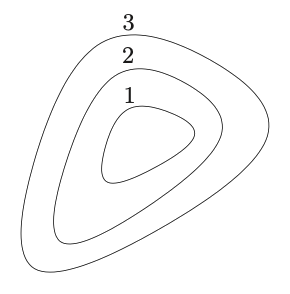
\includegraphics[width=0.25\textwidth]{images/fig1.png}
    \caption{Figure 1}
  \end{figure}
  Could $f$ be convex (concave, quasiconvex, quasiconcave)? Explain your answer. Repeat for the level curves shown below.
  \begin{figure}[H]
    \centering
    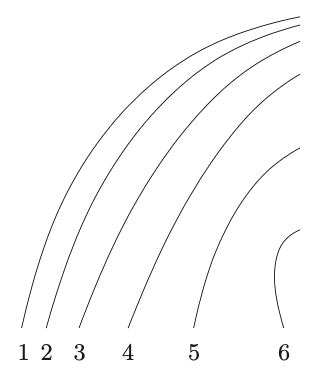
\includegraphics[width=0.25\textwidth]{images/fig2.png}
    \caption{Figure 2}
  \end{figure}

  \textbf{Solution:} For this question, we assume that the functions given uniformly grow or decay as depicted in the graphs without any abrupt changes in the function values. \\
  Based on this assumpption, the function in Figure 1 is probably quasiconvex since the 1, 2, and 3 sublevel sets are convex. It can also be possibly convex if the function grows upwards (hessian is positive semidefinite) from the center. This function can not be quasiconcave since the superlevel sets are not convex. Since it is not quasiconcave, it can not be concave either. \\
  The function in Figure 2 is probably quasiconcave since the 1, 2, and 3 superlevel sets are convex. It can also be possibly concave if grows downwards (hessian is negative semidefinite). This function can not be quasiconvex since the sublevel sets are not convex. Since it is not quasiconvex, it can not be convex either.

  \item[3.3] \textit{Inverse of an increasing convex function.} Suppose $f : \mathbb{R} \rightarrow \mathbb{R}$ is increasing and convex on its domain $(a, b)$. Let $g$ denote its inverse, i.e., the function with domain $(f(a), f(b))$ and $g(f(x)) = x$ for $a < x < b$. What can you say about convexity or concavity of $g$? \\
  
  \textbf{Solution:}
  \begin{align*}
    g(f(x)) &= x \\
    \Rightarrow g'(f(x)) f'(x) &= 1 \\
    \Rightarrow g'(f(x)) &= \frac{1}{f'(x)}
  \end{align*}
  Assuming that $f$ is strictly increasing, that is $f'(x) > 0$, we get $g'(y) > 0$. Now, substitute $y = f(x)$ or $x = g(y)$ to get:
  \begin{align*}
    g'(y) &= \frac{1}{f'(g(y))} \\
    \Rightarrow g''(y) &= -\frac{g'(y)}{f'(g(y))^2} \cdot f''(g(y)) \le 0
  \end{align*}
  Since $f$ is convex, hence $f''(g(y)) \ge 0$, and $g'(y) > 0$. Therefore, $g$ is concave.
\end{itemize}

\section{Convex Hulls}

\begin{itemize}
  \item[(a)] A vector $\mathbi{x} \in \mathbb{R}^n$ is 1-sparse if it has only one non-zero entry. What is the convex hull of all 1-sparse vectors in $\mathbb{R}^n$ with unit Euclidean norm? Justify your answer. \\
  
  \textbf{Solution:} 1-sparse vectors with unit Euclidean norm are the standard basis vectors $e_i$ (1 in the $i$th position and 0 everywhere else) and their negatives $-e_i$ in $\mathbb{R}^n$. Let $S = \{\pm e_1, \pm e_2, \dots, \pm e_n\}$. Now, we will prove that $\mathbf{conv} \, S$ is the unit $\ell_1$ norm ball centered at \textbf{0}, $B_1 = \{x \in \mathbb{R}^n : \|x\|_1 \le 1\}$. \\

  Proof: $\mathbf{conv} \, S \subseteq B_1$ \\
  We can easily see that $\|e_i\|_1 = 1 ~ \forall i$. Hence, $\pm e_i \in B_1 ~ \forall i$. Also, all $\ell_1$ norm balls are convex sets, and since the convex hull of a set is the intersection of all convex sets containing it, we get $\mathbf{conv} \, S \subseteq B_1$. \\

  Proof: $B_1 \subseteq \mathbf{conv} \, S$ \\
  Let $x \in B_1$. Now:
  \[ \|x\|_1 = \sum_{i=1}^n |x_i| \le 1 \]
  We can express $x$ as:
  \begin{align*}
    x &= \sum_{i=1}^n x_i e_i \\
    &= \sum_{i=1}^n |x_i| \cdot (\sgn(x_i) e_i) \tag{1}
  \end{align*}
  where $\sgn$ is the signum function defined as:
  \[ \sgn(x) = \begin{cases}
    1 & x \ge 0 \\
    -1 & x < 0
  \end{cases} \]
  $\sgn(0) = 1$ so that $\sgn(0) e_i \in S ~ \forall i$. Now, (1) is almost a convex combination of elements ($|x_i| \ge 0$) in $S$ except that the coefficients do not sum to 1 ($\sum_{i=1}^n |x_i| \le 1$). However, we can write:
  \begin{align*}
    x &= \sum_{i=1}^n |x_i| \cdot (\sgn(x_i) e_i) \\
    &= \sum_{i=1}^n |x_i| (\sgn(x_i) e_i) + \frac{1 - \sum_{i=1}^n |x_i|}{2} \cdot e_1 + \frac{1 - \sum_{i=1}^n |x_i|}{2} \cdot (-e_1)
  \end{align*}
  which makes the coefficients sum to 1. Hence, $x$ is a convex combination of elements in $S$, making it an element of $\mathbf{conv} \, S$. Therefore, $B_1 \subseteq \mathbf{conv} \, S$. \\

  Hence, we conclude that $\mathbf{conv} \, S = B_1$.
  
  \item[(b)] What is the convex hull of all orthogonal matrices? Justify your answer. \\
  
  \textbf{Solution:} Consider the vector space $\mathbb{R}^{n \times n}$ with the operator norm induced by the Euclidean norm, $\|\cdot\|_2$ defined as:
  \[ \|A\|_2 = \sup_{x \in \mathbb{R}^n} \frac{\|Ax\|_2}{\|x\|_2} \]
  Let $O(n)$ dentote the set of all orthogonal matrices in $\mathbb{R}^{n \times n}$. Since orthogonal matrices are isometries ($\|Ax\|_2 = \|x\|_2 ~ \forall x \in \mathbb{R}^n$), we have $\|A\|_2 = 1 ~ \forall A \in O(n)$. Intuitively, the convex hull of all orthogonal matrices seem to be the unit norm ball centered at \textbf{0} since all orthogonal matrices lie on the boundary of the unit norm ball. Let $B = \{A \in \mathbb{R}^n : \|A\|_2 \le 1\}$ be the unit norm ball. \\

  Proof: $\mathbf{conv} \, O(n) \subseteq B$ \\
  Since $\|A\|_2 = 1 ~ \forall A \in O(n)$, we know that $A \in B ~ \forall A \in O(n)$. Also, all norm balls are convex sets, and since the convex hull of a set is the intersection of all convex sets containing it, we get $\mathbf{conv} \, O(n) \subseteq B$. \\

  Proof: $B \subseteq \mathbf{conv} \, O(n)$ \\
  Let $A \in B$. Consider the singular value decomposition of $A$:
   \[ A = U \Sigma V^T \]
   where $U, V \in O(n)$ and $\Sigma = \mathbf{diag}(\sigma_1, \sigma_2, \dots, \sigma_n)$ with $\sigma_i$ being the singular values of $A$. Since the operator norm of $A$ is its largest singular value and $\|A\|_2 \le 1$, absolute values of entries of $\Sigma$ are bounded by 1. \\
   Define the $2^n$ diagonal matrices $\Sigma_i = \mathbf{diag}(\pm 1, \pm 1, \dots, \pm 1)$ by considering different combinations of $\pm 1$ for the diagonal entries. Note that $\Sigma$ lie in the convex hull of $\Sigma_i$ since it is a diagonal matrix with entries bounded by 1. Hence, we can write $\Sigma = \sum_{i=1}^{2^n} \alpha_i \Sigma_i$, where $\alpha_i \ge 0$ and $\sum_{i=1}^{2^n} \alpha_i = 1$. Now, we can write $A$ as:
   \begin{align*}
      A &= U \Sigma V^T \\
      &= U \left(\sum_{i=1}^{2^n} \alpha_i \Sigma_i\right) V^T \\
      &= \sum_{i=1}^{2^n} \alpha_i (U \Sigma_i V^T)
   \end{align*}
   Note that $\Sigma_i \Sigma_i^T = I ~ \forall i$ ($\Sigma_i$ are only made of $\pm 1$ on the diagonal), i.e. $\Sigma_i \in O(n) ~ \forall i$. Since $U, V \in O(n)$, we have $U \Sigma_i V^T \in O(n) ~ \forall i$. Hence, $A$ is a convex combination of orthogonal matrices, making it an element of $\mathbf{conv} \, O(n)$. Therefore, $B \subseteq \mathbf{conv} \, O(n)$. \\

   Combining the two results, we conclude that $\mathbf{conv} \, O(n) = B$.
\end{itemize}

\end{document}
